\documentclass[11pt]{article}

\usepackage[T1]{fontenc}
\usepackage[utf8]{inputenc}
\usepackage{lmodern}
\usepackage[letterpaper,margin=1.1in]{geometry}
\usepackage{amsmath,amssymb,amsthm}
\usepackage{microtype}
\usepackage{booktabs}
\usepackage{array}
\usepackage{tabularx}
\usepackage{enumitem}
\usepackage{xcolor}
\usepackage{tikz}
\usetikzlibrary{arrows.meta,calc}
\usepackage{caption}
\usepackage{subcaption}

\definecolor{linkblue}{HTML}{1F4FA8}
\definecolor{xc}{HTML}{1F5BC8}   % carries x
\definecolor{yc}{HTML}{C26B08}   % carries y
\definecolor{mc}{HTML}{7A3EBE}   % carries x + y
\definecolor{cc}{HTML}{4A505A}   % carrier bits
\definecolor{faint}{HTML}{C3C9D2}
\definecolor{colink}{HTML}{14808A}  % step 1: column links
\definecolor{rowlink}{HTML}{C0395E} % step 2: row links

\usepackage[colorlinks=true,linkcolor=linkblue,citecolor=linkblue,urlcolor=linkblue]{hyperref}
\hypersetup{pdftitle={Swap, Don't Route (written by Opus 5.5)}}

\captionsetup{font=small,labelfont=bf}
\captionsetup[sub]{font=small}

\newtheorem{theorem}{Theorem}
\newtheorem{lemma}[theorem]{Lemma}
\newtheorem{proposition}[theorem]{Proposition}
\newtheorem*{conjecture}{Conjecture}

\newcommand{\NC}{\mathrm{NC}}
\newcommand{\MCF}{\mathrm{MCF}}
\newcommand{\F}{\mathbb{F}_2}
\newcommand{\xeq}{\mathrel{\oplus\!\!=}}
\newcommand{\cx}[1]{\textcolor{xc}{#1}}
\newcommand{\cy}[1]{\textcolor{yc}{#1}}
\newcommand{\cm}[1]{\textcolor{mc}{#1}}
% \al{b}{j}{i}: the step-1 column carrier of column b that takes x_{jb} to p_{ib}
\newcommand{\al}[3]{\alpha_{#1,\,#2\to#3}}

\tikzset{
  nd/.style={circle, draw=black!85, fill=white, line width=0.55pt, minimum size=6.4mm, inner sep=0pt},
  ndsh/.style={nd, fill=black!10},
  arr/.style={-{Stealth[length=2.3mm,width=1.8mm]}, line width=1.1pt, shorten >=0.4pt, shorten <=0.4pt},
  ex/.style={arr, draw=xc},
  ey/.style={arr, draw=yc},
  em/.style={arr, draw=mc},
  ec/.style={arr, draw=cc},
  eco/.style={arr, draw=colink},
  fe/.style={line width=0.8pt, draw=faint},
  guide/.style={draw=black!22, line width=0.4pt, dash pattern=on 0.8pt off 2.2pt},
  lay/.style={font=\scriptsize, text=black!55},
  tag/.style={font=\scriptsize, text=black!70, fill=white, inner sep=1.2pt},
  badge/.style={circle, draw=black!85, fill=white, line width=0.5pt, inner sep=0pt, minimum size=3.9mm, font=\scriptsize\bfseries},
  ann/.style={font=\footnotesize, text=black!72, inner sep=1pt},
  % full-graph figure
  fg/.style={draw=black!38},
  fcol/.style={draw=colink},
  frow/.style={draw=rowlink},
  ftrunk/.style={draw=black!38, line width=2.6pt},
  cap1/.style={line width=0.5pt},
  cap2/.style={line width=1.0pt},
  cap3/.style={line width=1.5pt},
  box/.style={rectangle, rounded corners=2.5pt, draw=black!80, fill=white, line width=0.5pt, minimum width=6.2mm, minimum height=4.6mm, inner sep=1.2pt, font=\small},
  boxsh/.style={box, fill=black!10},
}

% One cell on its six layers: the t-lane O-H-p-R-t and the Z-lane s-C-q-G-Z.
% Shaded vertices are shared with other cells.
\newcommand{\cellbase}{%
  \foreach \l in {0,...,5} {
    \draw[guide] (-1.95,0.9*\l) -- (4.05,0.9*\l);
    \node[lay, anchor=east] at (-2.0,0.9*\l) {\l};
  }
  \node[lay, anchor=east] at (-2.0,5.0) {layer};
  \node[ndsh] (O) at (0,0)   {$O$};
  \node[ndsh] (H) at (0,0.9) {$H$};
  \node[nd]   (p) at (0,1.8) {$p$};
  \node[ndsh] (R) at (0,2.7) {$R$};
  \node[nd]   (t) at (0,3.6) {$t$};
  \node[nd]   (s) at (2.2,0.9) {$s$};
  \node[ndsh] (C) at (2.2,1.8) {$C$};
  \node[nd]   (q) at (2.2,2.7) {$q$};
  \node[ndsh] (G) at (2.2,3.6) {$G$};
  \node[ndsh] (Z) at (2.2,4.5) {$Z$};
  \node[tag, anchor=west] at ($(s.east)+(0.08,0)$) {source of $\cx{x}$};
  \node[tag, anchor=east] at ($(t.west)+(-0.08,0)$) {sink of $\cx{x}$};
  \node[tag, anchor=east] at ($(O.west)+(-0.08,0)$) {source of $\cy{y}$};
  \node[tag, anchor=west] at ($(Z.east)+(0.08,0)$) {sink of $\cy{y}$};
}

\title{Swap, Don't Route\\[4pt]
\large A 33-vertex counterexample to the undirected network coding conjecture\\[8pt]
\normalsize\textit{Written by Opus 5.5}}
\author{}
\date{Draft, October 7, 2026}

\begin{document}

\maketitle

\begin{abstract}
We describe a counterexample to the undirected network coding conjecture of Li and Li: a 33-vertex network on which an XOR code achieves rate~1 while routing achieves at most $149/150$. The network consists of six cells in a $3\times2$ grid. In each cell, two messages travel along short paths toward each other's sinks, and the three-step XOR swap exchanges the contents of the two paths. The first step is paid for once per column and the second once per row, each with a single parity bit, and the side information they need rides on extra messages whose shortest paths cross the same links anyway. The idea comes from the bit network of the preprint \emph{Integer multiplication below $n\log n$}~\cite{OAI26}. The same network also refutes a published theorem asserting that coding cannot lower the transmission cost in layered networks with uniform edge costs~\cite{XLWH14}.
\end{abstract}

\section{Introduction}

Consider an undirected network with integer edge capacities and a list of unicast sessions. In each session, a source must deliver independent message bits to a sink. \emph{Routing} treats bits as commodities: each bit travels along a path, and the paths share the capacity. The best common rate achievable this way is the maximum concurrent multicommodity flow, $\MCF$. \emph{Network coding} also lets intermediate vertices transmit functions of what they have received, such as XORs. We write $\NC$ for the best rate achievable with coding. Routing is a special case of coding, so $\NC\ge\MCF$.

In directed networks coding can beat routing by a wide margin, and the butterfly network is the standard example. In undirected networks the butterfly's advantage disappears, and Li and Li conjectured that coding never helps there~\cite{LL04}; see also~\cite{HKL06}. The conjecture is also known as the multiple-unicast conjecture.

\begin{conjecture}[undirected network coding conjecture]
For every undirected network with unicast sessions, $\NC=\MCF$.
\end{conjecture}

The conjecture has been proved for some restricted classes of networks (Section~\ref{sec:known}), and a recent preprint proves it for networks with at most five terminal locations~\cite{LQLL26}. It has also been used as a hypothesis for lower bounds. Assuming it, Afshani, Freksen, Kamma and Larsen proved that constant-degree Boolean circuits multiplying two $n$-bit integers need size $\Omega(n\log n)$~\cite{AFKL19}, and Farhadi, Hajiaghayi, Larsen and Shi proved lower bounds for sorting in external memory~\cite{FHLS19}.

\begin{theorem}\label{thm:main}
There is an undirected network $\mathcal N$ with $33$ vertices, $91$ edges and total capacity $149$, together with $30$ unit sessions on $7$ distinct source--sink pairs, such that
\[
\NC(\mathcal N)\;=\;1
\qquad\text{and}\qquad
\MCF(\mathcal N)\;\le\;\frac{149}{150}.
\]
\end{theorem}

Hence the conjecture is false. Braverman, Garg and Schvartzman showed that a single network on which coding beats routing can be amplified into a family of networks on which $\NC/\MCF\ge(\log|V|)^c$ for a constant $c>0$, where $|V|$ is the number of vertices~\cite{BGS17}. Applied to $\mathcal N$, their result shows that, in the words of their title, network coding in undirected graphs is very helpful. The lower bounds of~\cite{AFKL19,FHLS19} assumed the conjecture; the counterexample refutes that assumption but does not show that the bounds themselves fail.

Deleting the hub $O$ and letting each bit it sends start at its recipient instead gives a 32-vertex network with $\MCF\le125/126$, at the cost of 13 distinct source--sink pairs instead of~7 (Appendix~\ref{app:32}).

Section~\ref{sec:known} compares $\mathcal N$ with the classes of networks on which the conjecture has been proved (Table~\ref{tab:known}). It also shows that $\mathcal N$ refutes Theorem~6.3 of Xiahou, Li, Wu and Huang~\cite{XLWH14}, which asserts that in a layered network with uniform edge costs, where each session's source and sink lie in different layers, no code meets the sessions' rates more cheaply than routing does.

\paragraph{Origin.} The construction comes from a recent preprint that claims an integer multiplication algorithm running in time $O(n(\log n)^{1-\kappa})$, for some constant $\kappa>0$, on a multitape Turing machine~\cite{OAI26}. The counterexample does not rely on the multiplication result being correct. The algorithm's engine is a fast way to permute data on tape. The paper observes in its Section~1.7 that this procedure ``forms XOR combinations of intermediate data, even though its final effect is a permutation.'' A permutation is pure data movement, so the procedure uses coding where one would expect routing. Section~\ref{sec:idea} turns the XOR swap at its core into a network where coding beats routing, and ends by tracing the correspondence.

\paragraph{Model.} Edges are undirected, and capacities bound traffic in both directions together; in all other respects we follow the standard model of Braverman, Garg and Schvartzman~\cite[\S2 and Appendix~A]{BGS17}. Several sessions may share endpoints, so the $30$ unit sessions of Theorem~\ref{thm:main} amount to $7$ sessions: one from $O$ to $Z$ with demand $24$, and six from $s_{ab}$ to $t_{ab}$ with demand~$1$. Appendix~\ref{app:variants} gives variants in which every session has its own endpoints or every capacity is~1. Our code delivers one bit per session with a fixed causal schedule of XORs that stays within every capacity, so it achieves rate~1.

\paragraph{Verification.} Two scripts in the accompanying repository check the construction exactly, using only Python's standard library. Gaussian elimination over $\F$ confirms that every sender can compute each bit it sends and that every sink can decode, and the scripts also check every capacity, the layer structure and all hop distances. The script \texttt{scripts/verify-network-coding-33.py} checks $\mathcal N$, and \texttt{scripts/verify-network-coding-32.py} checks the 32-vertex version.

\section{The idea: swap, don't route}\label{sec:idea}

\paragraph{The XOR swap.} Over $\F$, three XOR updates exchange two values:
\[
(x,\,y)\;\longmapsto\;(x,\;x\oplus y)\;\longmapsto\;(y,\;x\oplus y)\;\longmapsto\;(y,\;x).
\]
Read this as a network. One path carries $x$ and another carries $y$, and each update sends one bit from one path to the other. After the three updates the first path holds $y$ and the second holds $x$. Neither bit is routed along the other path; the paths only trade contents.

\paragraph{Why this can beat routing.} Suppose that $x$ must go from $s$ to $t$ and $y$ from $O$ to $Z$, but the short paths in the network join $s$ to $Z$ and $O$ to $t$. Routing must still send each bit to its own sink. Coding can send $x$ toward $Z$ and $y$ toward $t$ along the short paths and then swap the contents with three XOR updates between the two paths. This wins if the updates cost less than routing's detours.

\paragraph{One cell.} Our network consists of six \emph{cells} arranged in a $3\times2$ grid, with three rows and two columns, and each cell has its own pair of messages $x$ and $y$. Figure~\ref{fig:cell} shows one cell, with subscripts dropped. The vertices lie in six layers, and every edge joins two consecutive layers. Call a path \emph{monotone} if each of its edges goes up one layer. The \emph{$t$-lane} $O\to H\to p\to R\to t$ and the \emph{$Z$-lane} $s\to C\to q\to G\to Z$, named for where they end, are monotone paths of 4 hops each. No path from $s$ to $t$ is monotone (Lemma~\ref{lem:monotone}), so routing $x$ needs a detour, 5 hops to climb 3 layers, while $y$ needs 5 hops to climb 5 layers. Counting one \emph{bit-hop} per bit per edge, routing a cell costs 10 while the lanes cost 8, so the swap can save up to 2 bit-hops per cell.

Only $s$, $p$, $q$ and $t$ belong to the cell, and Figure~\ref{fig:cell} shades the other vertices. The \emph{column parity vertex} $C$ is shared by the three cells of its column, the \emph{row parity vertex} $R$ by the two cells of its row, and the hubs $O$, $H$, $G$ and $Z$ by all six cells. This sharing is what makes the swap affordable.

\begin{figure}[ht]
\centering
\begin{subfigure}[t]{0.49\linewidth}
\centering
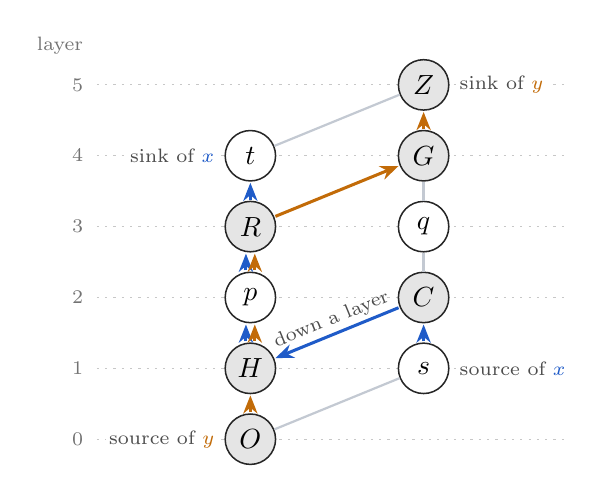
\begin{tikzpicture}
\cellbase
\draw[fe] (O) -- (s);  \draw[fe] (C) -- (q);  \draw[fe] (q) -- (G);  \draw[fe] (Z) -- (t);
\draw[ex] (s) -- (C);
\draw[ex] (C) -- node[sloped, above, font=\scriptsize, text=black!70, inner sep=1.5pt] {down a layer} (H);
\draw[ex] ([xshift=-1.6pt]H.north) -- ([xshift=-1.6pt]p.south);
\draw[ex] ([xshift=-1.6pt]p.north) -- ([xshift=-1.6pt]R.south);
\draw[ex] (R) -- (t);
\draw[ey] (O) -- (H);
\draw[ey] ([xshift=1.6pt]H.north) -- ([xshift=1.6pt]p.south);
\draw[ey] ([xshift=1.6pt]p.north) -- ([xshift=1.6pt]R.south);
\draw[ey] (R) -- (G);
\draw[ey] (G) -- (Z);
\end{tikzpicture}
\caption{Routing: 10 bit-hops per cell.}
\end{subfigure}\hfill
\begin{subfigure}[t]{0.49\linewidth}
\centering
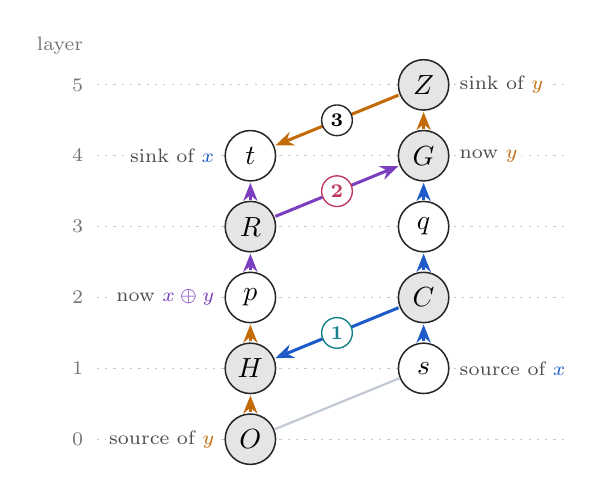
\begin{tikzpicture}
\cellbase
\node[tag, anchor=east] at ($(p.west)+(-0.08,0)$) {now $\cm{x\oplus y}$};
\node[tag, anchor=west] at ($(G.east)+(0.08,0)$) {now $\cy{y}$};
\draw[fe] (O) -- (s);
\draw[ex] (s) -- (C);  \draw[ex] (C) -- (q);  \draw[ex] (q) -- (G);  \draw[ey] (G) -- (Z);
\draw[ey] (O) -- (H);  \draw[ey] (H) -- (p);  \draw[em] (p) -- (R);  \draw[em] (R) -- (t);
\draw[ex] (C) -- node[badge, draw=colink, text=colink] {1} (H);
\draw[em] (R) -- node[badge, draw=rowlink, text=rowlink] {2} (G);
\draw[ey] (Z) -- node[badge] {3} (t);
\end{tikzpicture}
\caption{Coding: 9 bit-hops per cell, plus parities.}
\end{subfigure}
\caption{One cell $(a,b)$ of $\mathcal N$ with its subscripts dropped. Shaded vertices are shared with other cells. Link colors show what each link carries: \cx{blue} for $x$, \cy{orange} for $y$ and \cm{violet} for $x\oplus y$. Gray links belong to the network but are not used for $x$ or $y$ in that panel. (a)~No path from $s$ to $t$ is monotone, so $x$ needs 5 hops to climb 3 layers. (b)~$x$ rides the $Z$-lane and $y$ the $t$-lane, and three XOR steps swap their contents. Step~1 costs one bit per column and step~2 one bit per row; only step~3 is paid for per cell. In every figure, \textcolor{colink}{teal} marks step~1 and \textcolor{rowlink}{rose} marks step~2.}
\label{fig:cell}
\end{figure}

\paragraph{Paying for the swap.} Each XOR update needs a bit to cross between the lanes. If every cell paid for its own three crossings, coding would cost $8+3=11$ bit-hops per cell and lose. We call the three updates steps~1, 2 and~3. The construction pays for step~3 directly, with one hop $Z\to t$ per cell, and pays for the first two steps in bulk:
\begin{itemize}[nosep]
\item Step~1 ($y\xeq x$) is done for a whole column at once. One parity bit per column crosses from the $Z$-lane to the $t$-lane, along $C\to H$.
\item Step~2 ($x\xeq y$) is done for a whole row at once. One parity bit per row crosses back, along $R\to G$.
\end{itemize}
Each cell then recovers its own term from the parity. In step~1, for instance, a cell that knows the other bits of its column can cancel them from the column parity, leaving its own.

\paragraph{Side information at no extra cost.} The parity trick needs side information: to cancel the other cells' bits, a cell must receive bits that contain them. These bits travel on \emph{cross-cell links}, which join vertices of different cells: \emph{column links}, within a column, serve step~1, and \emph{row links}, within a row, serve step~2. In an undirected network, a link that coding spends on side information is usually one that routing could use to carry the message itself, which is why the butterfly's gain disappears. Here every side-information bit piggybacks on a \emph{carrier}, an extra message from $O$ to $Z$ that crosses that link anyway, on one of its shortest paths (Figure~\ref{fig:carrier}): \emph{column carriers} cross column links and \emph{row carriers} cross row links. Routing must pay for the carriers too, so it gains nothing from the cross-cell links. Each carrier travels exactly its distance, so carriers cost the same under coding as under routing.

\begin{figure}[t]
\centering
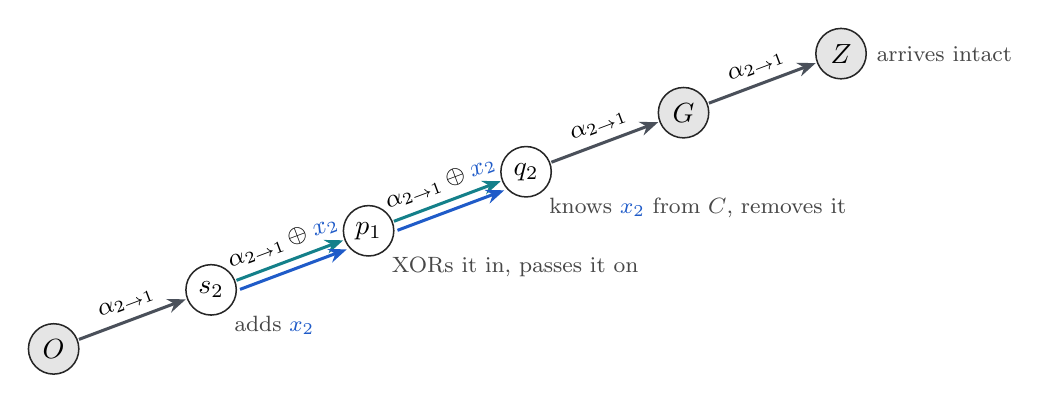
\begin{tikzpicture}
\node[ndsh] (O) at (0,0)    {$O$};
\node[nd] (s2)  at (2,0.75) {$s_2$};
\node[nd] (p1)  at (4,1.5)  {$p_1$};
\node[nd] (q2)  at (6,2.25) {$q_2$};
\node[ndsh] (G) at (8,3.0)  {$G$};
\node[ndsh] (Z) at (10,3.75){$Z$};
\draw[ec]  (O)  -- node[sloped, above, font=\small] {$\alpha_{2\to1}$} (s2);
\draw[eco] (s2) -- node[sloped, above, font=\small] {$\alpha_{2\to1}\oplus\cx{x_2}$} (p1);
\draw[eco] (p1) -- node[sloped, above, font=\small] {$\alpha_{2\to1}\oplus\cx{x_2}$} (q2);
\draw[ec]  (q2) -- node[sloped, above, font=\small] {$\alpha_{2\to1}$} (G);
\draw[ec]  (G)  -- node[sloped, above, font=\small] {$\alpha_{2\to1}$} (Z);
\draw[ex, transform canvas={shift={(0.045,-0.115)}}] (s2) -- (p1);
\draw[ex, transform canvas={shift={(0.045,-0.115)}}] (p1) -- (q2);
\node[ann, anchor=north west] at ($(s2.south east)+(0.02,-0.06)$) {adds $\cx{x_2}$};
\node[ann, anchor=north west] at ($(p1.south east)+(0.02,-0.06)$) {XORs it in, passes it on};
\node[ann, anchor=north west] at ($(q2.south east)+(0.02,-0.06)$) {knows $\cx{x_2}$ from $C$, removes it};
\node[ann, anchor=west] at ($(Z.east)+(0.08,0)$) {arrives intact};
\end{tikzpicture}
\caption{The column carrier $\alpha_{2\to1}$, with the column index dropped. It follows a monotone path from $O$ to $Z$, five hops in all, which is exactly its distance. On its two column links (\textcolor{colink}{teal}, as in Figure~\ref{fig:full}) it also carries $x_2$. The vertex $p_1$ uses this bit in its own XOR and forwards it unchanged. The vertex $q_2$ already knows $x_2$ because $C$ sent it there, so it removes $x_2$, and the carrier arrives intact.}
\label{fig:carrier}
\end{figure}

\paragraph{The count.} Per cell, swapping saves the 2-hop detour and spends 1 hop on step~3. Step~1 costs one parity bit per column and step~2 one per row, and carriers cost what they would under routing. So routing needs more bit-hops than coding uses, by
\[
\text{cells}-\text{rows}-\text{columns}\;=\;6-3-2\;=\;1,
\]
which gives 149 bit-hops against 150 (Table~\ref{tab:count}). This comparison is not a heuristic; it is the routing bound. The capacity of each edge is defined as the number of bits the code sends across it, so the total capacity equals coding's bit-hop count, while routing at rate~1 must spend at least the sum of the sessions' distances (Section~\ref{sec:routing}).

To see what the count gives for other shapes, view the set of cells as a bipartite graph with a vertex for each row and each column and an edge for each cell. When this graph is connected, the saving $\text{cells}-\text{rows}-\text{columns}$ is one less than its cycle rank, so the count favors coding exactly when the graph has at least two independent cycles. $K_{2,3}$, our $3\times2$ grid, is the smallest bipartite graph with two. A count of zero or less does not by itself rule out a gap, but for the $2\times2$ grid an LP solve confirms that there is none. Appendix~\ref{app:other} gives the count for any grid.

\paragraph{Where the idea comes from.} At the core of the procedure of~\cite{OAI26} is a fixed linear network, the \emph{bit network} of its Section~3, which swaps two banks of bits with the same three steps $y\xeq x$, $x\xeq y$, $y\xeq x$, but performs each step indirectly: central wires gather sums of many values, each target adds in the sums it needs, and side wires carry copies of neighboring values that cancel the unwanted terms, a cancellation the paper relates to linear index coding~\cite{BBJK06}. Its scratch wires may start with arbitrary contents and are restored at the end, which the paper traces to catalytic computation~\cite{BCKLS14}. In $\mathcal N$ the central wires become the parity bits, the side wires become the cross-cell links, and ``restored'' becomes ``delivered'': a scratch value that must come back intact behaves like a carrier, a message that must arrive intact.

\begin{table}[ht]
\centering
\begin{tabular}{@{}l r r@{}}
\toprule
Item & Coding & Routing\\
\midrule
$x$ and $y$ of one cell & 9 & at least 10\\
One carrier & 5 & at least 5\\
One column parity & 1 & not needed\\
One row parity & 1 & not needed\\
\midrule
Whole $3\times2$ grid: $6$ cells, $18$ carriers, $2$ columns, $3$ rows & 149 & at least 150\\
\bottomrule
\end{tabular}
\caption{Capacity used by coding and needed by routing, in bit-hops.}
\label{tab:count}
\end{table}

\section{The network and the code}\label{sec:construction}

The six cells $(a,b)$ form a $3\times2$ grid, with rows indexed by $a\in\{1,2,3\}$ and columns by $b\in\{1,2\}$. We write $\bar b=3-b$ for the other column. All sums are XORs over $\F$.

\paragraph{Vertices.} Each cell $(a,b)$ has four vertices $s_{ab}$, $p_{ab}$, $q_{ab}$ and $t_{ab}$. Each column $b$ has a column parity vertex $C_b$, each row $a$ has a row parity vertex $R_a$, and there are four hubs $O$, $H$, $G$ and $Z$, for 33 vertices in all. Layer~0 holds $O$, layer~1 holds $H$ and the $s_{ab}$, layer~2 the $C_b$ and $p_{ab}$, layer~3 the $R_a$ and $q_{ab}$, layer~4 $G$ and the $t_{ab}$, and layer~5 holds $Z$.

\paragraph{Messages.} There are 30 independent message bits: $x_{ab}$ from $s_{ab}$ to $t_{ab}$, $y_{ab}$ from $O$ to $Z$, and carriers from $O$ to $Z$. For each column $b$ and each ordered pair of distinct rows $(j,i)$, the column carrier $\al{b}{j}{i}$ will take $x_{jb}$ to $p_{ib}$ in step~1. For each cell $(a,b)$, the row carrier $\beta_{ab}$ will take $x_{ab}\oplus y_{ab}$ to $q_{a\bar b}$ in step~2.

\paragraph{Edges.} The edges of $\mathcal N$ are exactly the links the code uses, and the capacity $c_e$ of an edge $e$ is the number of bits the code sends across it, in both directions together. Figure~\ref{fig:full} draws the result, which has 91 edges and total capacity~149. Step~1 uses the column links and step~2 the row links. Appendix~\ref{app:spec} lists every message, transmission and edge.

\begin{figure}[t]
\centering
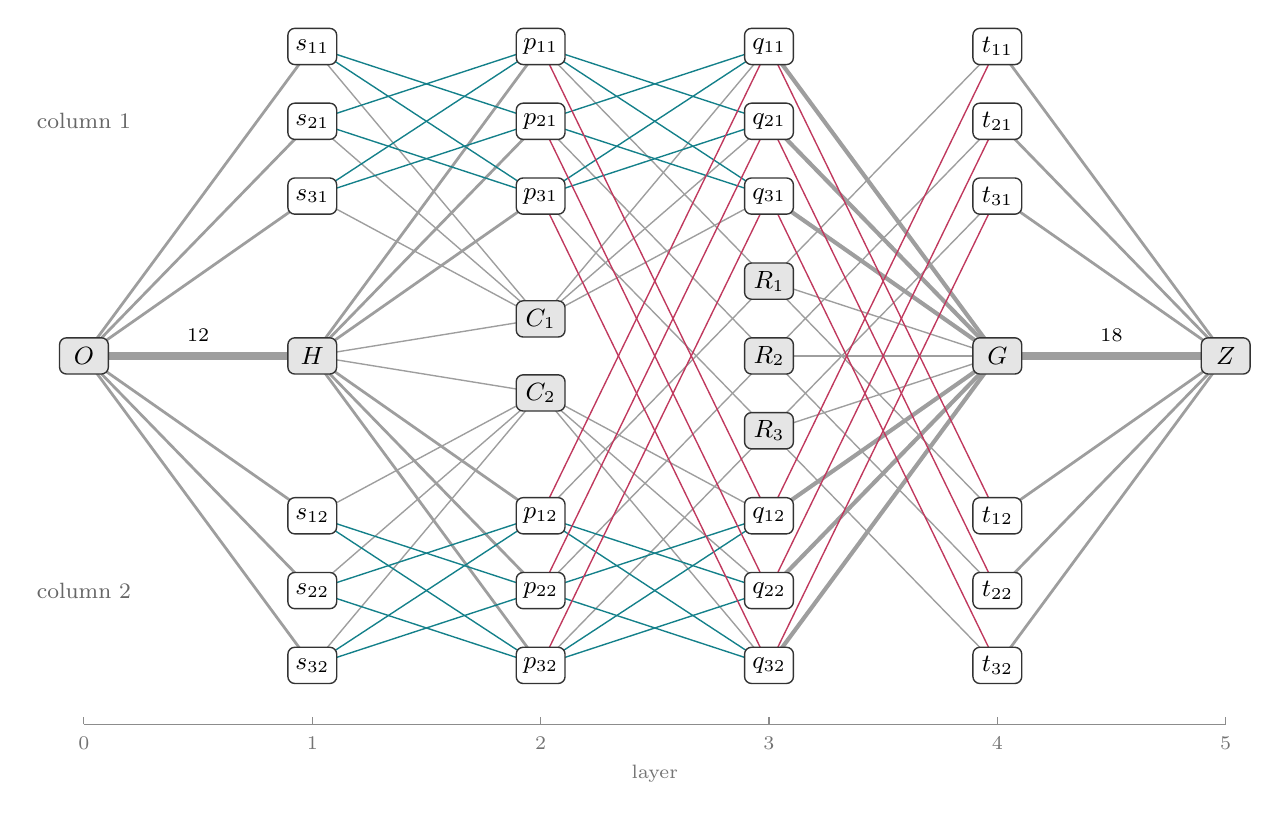
\begin{tikzpicture}[x=1cm,y=1cm]
\coordinate (O) at (0.00,0.00);
\coordinate (s11) at (2.90,3.93);
\coordinate (s21) at (2.90,2.98);
\coordinate (s31) at (2.90,2.03);
\coordinate (H) at (2.90,0.00);
\coordinate (s12) at (2.90,-2.03);
\coordinate (s22) at (2.90,-2.98);
\coordinate (s32) at (2.90,-3.93);
\coordinate (p11) at (5.80,3.93);
\coordinate (p21) at (5.80,2.98);
\coordinate (p31) at (5.80,2.03);
\coordinate (C1) at (5.80,0.47);
\coordinate (C2) at (5.80,-0.47);
\coordinate (p12) at (5.80,-2.03);
\coordinate (p22) at (5.80,-2.98);
\coordinate (p32) at (5.80,-3.93);
\coordinate (q11) at (8.70,3.93);
\coordinate (q21) at (8.70,2.98);
\coordinate (q31) at (8.70,2.03);
\coordinate (D1) at (8.70,0.95);
\coordinate (D2) at (8.70,0.00);
\coordinate (D3) at (8.70,-0.95);
\coordinate (q12) at (8.70,-2.03);
\coordinate (q22) at (8.70,-2.98);
\coordinate (q32) at (8.70,-3.93);
\coordinate (t11) at (11.60,3.93);
\coordinate (t21) at (11.60,2.98);
\coordinate (t31) at (11.60,2.03);
\coordinate (G) at (11.60,0.00);
\coordinate (t12) at (11.60,-2.03);
\coordinate (t22) at (11.60,-2.98);
\coordinate (t32) at (11.60,-3.93);
\coordinate (Z) at (14.50,0.00);
\draw[fg, cap1] (C1) -- (q11);
\draw[fg, cap1] (C1) -- (q21);
\draw[fg, cap1] (C1) -- (q31);
\draw[fg, cap1] (C2) -- (q12);
\draw[fg, cap1] (C2) -- (q22);
\draw[fg, cap1] (C2) -- (q32);
\draw[fg, cap1] (D1) -- (G);
\draw[fg, cap1] (D1) -- (t11);
\draw[fg, cap1] (D1) -- (t12);
\draw[fg, cap1] (D2) -- (G);
\draw[fg, cap1] (D2) -- (t21);
\draw[fg, cap1] (D2) -- (t22);
\draw[fg, cap1] (D3) -- (G);
\draw[fg, cap1] (D3) -- (t31);
\draw[fg, cap1] (D3) -- (t32);
\draw[fg, cap1] (H) -- (C1);
\draw[fg, cap1] (H) -- (C2);
\draw[fg, cap1] (p11) -- (D1);
\draw[fg, cap1] (p12) -- (D1);
\draw[fg, cap1] (p21) -- (D2);
\draw[fg, cap1] (p22) -- (D2);
\draw[fg, cap1] (p31) -- (D3);
\draw[fg, cap1] (p32) -- (D3);
\draw[fg, cap1] (s11) -- (C1);
\draw[fg, cap1] (s12) -- (C2);
\draw[fg, cap1] (s21) -- (C1);
\draw[fg, cap1] (s22) -- (C2);
\draw[fg, cap1] (s31) -- (C1);
\draw[fg, cap1] (s32) -- (C2);
\draw[fg, cap2] (H) -- (p11);
\draw[fg, cap2] (H) -- (p12);
\draw[fg, cap2] (H) -- (p21);
\draw[fg, cap2] (H) -- (p22);
\draw[fg, cap2] (H) -- (p31);
\draw[fg, cap2] (H) -- (p32);
\draw[fg, cap2] (O) -- (s11);
\draw[fg, cap2] (O) -- (s12);
\draw[fg, cap2] (O) -- (s21);
\draw[fg, cap2] (O) -- (s22);
\draw[fg, cap2] (O) -- (s31);
\draw[fg, cap2] (O) -- (s32);
\draw[fg, cap2] (t11) -- (Z);
\draw[fg, cap2] (t12) -- (Z);
\draw[fg, cap2] (t21) -- (Z);
\draw[fg, cap2] (t22) -- (Z);
\draw[fg, cap2] (t31) -- (Z);
\draw[fg, cap2] (t32) -- (Z);
\draw[fg, cap3] (q11) -- (G);
\draw[fg, cap3] (q12) -- (G);
\draw[fg, cap3] (q21) -- (G);
\draw[fg, cap3] (q22) -- (G);
\draw[fg, cap3] (q31) -- (G);
\draw[fg, cap3] (q32) -- (G);
\draw[fcol, cap1] (p11) -- (q21);
\draw[fcol, cap1] (p11) -- (q31);
\draw[fcol, cap1] (p12) -- (q22);
\draw[fcol, cap1] (p12) -- (q32);
\draw[fcol, cap1] (p21) -- (q11);
\draw[fcol, cap1] (p21) -- (q31);
\draw[fcol, cap1] (p22) -- (q12);
\draw[fcol, cap1] (p22) -- (q32);
\draw[fcol, cap1] (p31) -- (q11);
\draw[fcol, cap1] (p31) -- (q21);
\draw[fcol, cap1] (p32) -- (q12);
\draw[fcol, cap1] (p32) -- (q22);
\draw[fcol, cap1] (s11) -- (p21);
\draw[fcol, cap1] (s11) -- (p31);
\draw[fcol, cap1] (s12) -- (p22);
\draw[fcol, cap1] (s12) -- (p32);
\draw[fcol, cap1] (s21) -- (p11);
\draw[fcol, cap1] (s21) -- (p31);
\draw[fcol, cap1] (s22) -- (p12);
\draw[fcol, cap1] (s22) -- (p32);
\draw[fcol, cap1] (s31) -- (p11);
\draw[fcol, cap1] (s31) -- (p21);
\draw[fcol, cap1] (s32) -- (p12);
\draw[fcol, cap1] (s32) -- (p22);
\draw[frow, cap1] (p11) -- (q12);
\draw[frow, cap1] (p12) -- (q11);
\draw[frow, cap1] (p21) -- (q22);
\draw[frow, cap1] (p22) -- (q21);
\draw[frow, cap1] (p31) -- (q32);
\draw[frow, cap1] (p32) -- (q31);
\draw[frow, cap1] (q11) -- (t12);
\draw[frow, cap1] (q12) -- (t11);
\draw[frow, cap1] (q21) -- (t22);
\draw[frow, cap1] (q22) -- (t21);
\draw[frow, cap1] (q31) -- (t32);
\draw[frow, cap1] (q32) -- (t31);
\draw[ftrunk] (O) -- (H);
\draw[ftrunk] (G) -- (Z);
\node[font=\scriptsize, above=1.5pt] at ($(O)!0.5!(H)$) {12};
\node[font=\scriptsize, above=1.5pt] at ($(G)!0.5!(Z)$) {18};
\node[boxsh] at (O) {$O$};
\node[box] at (s11) {$s_{11}$};
\node[box] at (s21) {$s_{21}$};
\node[box] at (s31) {$s_{31}$};
\node[boxsh] at (H) {$H$};
\node[box] at (s12) {$s_{12}$};
\node[box] at (s22) {$s_{22}$};
\node[box] at (s32) {$s_{32}$};
\node[box] at (p11) {$p_{11}$};
\node[box] at (p21) {$p_{21}$};
\node[box] at (p31) {$p_{31}$};
\node[boxsh] at (C1) {$C_{1}$};
\node[boxsh] at (C2) {$C_{2}$};
\node[box] at (p12) {$p_{12}$};
\node[box] at (p22) {$p_{22}$};
\node[box] at (p32) {$p_{32}$};
\node[box] at (q11) {$q_{11}$};
\node[box] at (q21) {$q_{21}$};
\node[box] at (q31) {$q_{31}$};
\node[boxsh] at (D1) {$R_{1}$};
\node[boxsh] at (D2) {$R_{2}$};
\node[boxsh] at (D3) {$R_{3}$};
\node[box] at (q12) {$q_{12}$};
\node[box] at (q22) {$q_{22}$};
\node[box] at (q32) {$q_{32}$};
\node[box] at (t11) {$t_{11}$};
\node[box] at (t21) {$t_{21}$};
\node[box] at (t31) {$t_{31}$};
\node[boxsh] at (G) {$G$};
\node[box] at (t12) {$t_{12}$};
\node[box] at (t22) {$t_{22}$};
\node[box] at (t32) {$t_{32}$};
\node[boxsh] at (Z) {$Z$};
\node[font=\footnotesize, text=black!60] at (0,2.98) {column 1};
\node[font=\footnotesize, text=black!60] at (0,-2.98) {column 2};
\draw[black!45, line width=0.4pt] (0,-4.68) -- (14.50,-4.68);
\draw[black!45, line width=0.4pt] (0.00,-4.68) -- ++(0,0.1);
\node[lay, below=1pt] at (0.00,-4.68) {0};
\draw[black!45, line width=0.4pt] (2.90,-4.68) -- ++(0,0.1);
\node[lay, below=1pt] at (2.90,-4.68) {1};
\draw[black!45, line width=0.4pt] (5.80,-4.68) -- ++(0,0.1);
\node[lay, below=1pt] at (5.80,-4.68) {2};
\draw[black!45, line width=0.4pt] (8.70,-4.68) -- ++(0,0.1);
\node[lay, below=1pt] at (8.70,-4.68) {3};
\draw[black!45, line width=0.4pt] (11.60,-4.68) -- ++(0,0.1);
\node[lay, below=1pt] at (11.60,-4.68) {4};
\draw[black!45, line width=0.4pt] (14.50,-4.68) -- ++(0,0.1);
\node[lay, below=1pt] at (14.50,-4.68) {5};
\node[lay] at (7.25,-5.30) {layer};
\end{tikzpicture}
\caption{The full network $\mathcal N$, drawn by layer from left to right. Column~1 of the grid is drawn above the hubs and column~2 below, with rows 1 to 3 from top to bottom, so the vertices $s_{ab},p_{ab},q_{ab},t_{ab}$ of each cell lie on one horizontal line. Shaded vertices are shared between cells. \textcolor{colink}{Teal}: column links, used in step~1, $s_{jb}p_{ib}$ and $p_{ib}q_{jb}$ ($j\neq i$), which carry $\al{b}{j}{i}\oplus x_{jb}$. \textcolor{rowlink}{Rose}: row links, used in step~2, $p_{ab}q_{a\bar b}$ and $q_{a\bar b}t_{ab}$, which carry $\beta_{ab}\oplus x_{ab}\oplus y_{ab}$. Gray: every other edge, including the parity links $C_bH$ and $R_aG$. Line width grows with capacity: the edges $Os_{ab}$, $Hp_{ab}$ and $t_{ab}Z$ have capacity~2, the edges $q_{ab}G$ have capacity~3, $OH$ and $GZ$ have the capacities shown, and every other edge has capacity~1.}
\label{fig:full}
\end{figure}

\subsection{Step 1: \texorpdfstring{$y\xeq x$}{y ^= x}, one column at a time}\label{sec:r1}

Fix a column $b$.
\begin{itemize}[nosep]
\item Each $s_{ab}$ sends $x_{ab}$ up the $Z$-lane to $C_b$, which forwards it to $q_{ab}$ and sends the column parity $P_b=x_{1b}\oplus x_{2b}\oplus x_{3b}$ down to $H$.
\item $O$ sends $y_{ab}\oplus\sum_{j\neq a}\al{b}{j}{a}$ to $H$, which adds $P_b$ and sends the result, $u_{ab}$, up the $t$-lane to $p_{ab}$.
\item For each ordered pair of distinct rows $(j,i)$, $O$ sends the column carrier $\al{b}{j}{i}$ to $s_{jb}$. The vertex $s_{jb}$ sends $\al{b}{j}{i}\oplus x_{jb}$ along a column link to $p_{ib}$, which passes it on to $q_{jb}$.
\end{itemize}
The vertex $p_{ab}$ XORs what it has received,
\[
u_{ab}\oplus\sum_{j\neq a}\bigl(\al{b}{j}{a}\oplus x_{jb}\bigr)
\;=\;y_{ab}\oplus P_b\oplus\sum_{j\neq a}x_{jb}
\;=\;y_{ab}\oplus x_{ab},
\]
which we call $w_{ab}$. The vertex $q_{jb}$ knows $x_{jb}$ from $C_b$, so it strips $x_{jb}$ from each carrier it receives and sends $\al{b}{j}{i}$ through $G$ to $Z$.

\subsection{Step 2: \texorpdfstring{$x\xeq y$}{x ^= y}, one row at a time}\label{sec:r2}

Fix a row $a$. It has two cells, $(a,1)$ and $(a,2)$, and after step~1 each $p_{ab}$ holds $w_{ab}$.
\begin{itemize}[nosep]
\item Each $p_{ab}$ sends $w_{ab}$ up the $t$-lane to $R_a$, which forwards it to $t_{ab}$ and sends the row parity $Q_a=w_{a1}\oplus w_{a2}$ up to $G$.
\item $O$ sends the row carrier $\beta_{ab}$ through $H$ to $p_{ab}$, which sends $v_{ab}=\beta_{ab}\oplus w_{ab}$ along a row link to $q_{a\bar b}$. That vertex passes $v_{ab}$ on to $t_{ab}$, which knows $w_{ab}$ from $R_a$, removes it, and sends $\beta_{ab}$ to $Z$.
\item Each $q_{ab}$ knows $x_{ab}$ from step~1 and has received $v_{a\bar b}$, so it sends $F_{ab}=x_{ab}\oplus v_{a\bar b}$ up to $G$.
\end{itemize}
The hub $G$ adds the row parity and sends
\[
F_{ab}\oplus Q_a
\;=\;x_{ab}\oplus\beta_{a\bar b}\oplus w_{a\bar b}\oplus w_{a1}\oplus w_{a2}
\;=\;x_{ab}\oplus w_{ab}\oplus\beta_{a\bar b}
\;=\;y_{ab}\oplus\beta_{a\bar b}
\]
to $Z$. The hub $Z$ has received $\beta_{a\bar b}$ from $t_{a\bar b}$, so it recovers $y_{ab}$.

\subsection{Step 3: \texorpdfstring{$y\xeq x$}{y ^= x}, one hop per cell}\label{sec:r3}

$Z$ sends $y_{ab}$ down to $t_{ab}$, which holds $w_{ab}$ from step~2 and computes $x_{ab}=w_{ab}\oplus y_{ab}$.

\begin{proposition}\label{prop:code}
The code of Sections~\ref{sec:r1}--\ref{sec:r3}, listed in full in Table~\ref{tab:protocol}, is causal and zero-error, has block length~1, delivers every message bit to its sink, and sends exactly $c_e$ bits across each edge $e$. Hence $\NC(\mathcal N)=1$.
\end{proposition}

\begin{proof}
Table~\ref{tab:protocol} lists the transmissions of the three steps in a causal order: each sender already knows every bit it sends. Sections~\ref{sec:r1}--\ref{sec:r3} show the computations, and Table~\ref{tab:lanes} traces them hop by hop for one cell. At the end $Z$ holds every $y$, $\alpha$ and $\beta$ bit, and each $t_{ab}$ holds $x_{ab}$. The capacities were defined as the code's traffic, so every edge carries exactly its capacity. Hence $\NC(\mathcal N)\ge1$.

Conversely, the edges at $O$ are $OH$, of capacity $12$, and the six edges $Os_{ab}$, of capacity $2$ each, for a total of $24$. The $24$ sessions from $O$ to $Z$ must all cross this cut, so by the cut bound, which holds for coding as well as routing, $\NC(\mathcal N)\le1$.
\end{proof}

\section{Routing needs capacity 150}\label{sec:routing}

Recall that a path is monotone if each of its edges goes up one layer. Every edge joins two consecutive layers, so a path that goes down a layer on $d$ of its edges is $2d$ edges longer than the difference between the layers of its endpoints.

\begin{lemma}\label{lem:monotone}
For every cell $(a,b)$, no path from $s_{ab}$ to $t_{ab}$ is monotone. Hence every such path has at least $5$ edges.
\end{lemma}

\begin{proof}
A monotone path from $s_{ab}$ in layer~1 to $t_{ab}$ in layer~4 has exactly three edges, so it consists of $s_{ab}$, a vertex in layer~2, a vertex in layer~3, and $t_{ab}$. The layer-2 vertex is a neighbor of $s_{ab}$, so it is $C_b$ or $p_{ib}$ with $i\neq a$, and the layer-3 vertex is a neighbor of $t_{ab}$, so it is $R_a$ or $q_{a\bar b}$. Among the vertices of layer~3, however, $C_b$ is adjacent only to the $q_{kb}$, and $p_{ib}$ only to $R_i$, to the $q_{kb}$ with $k\neq i$, and to $q_{i\bar b}$. None of these is $R_a$ or $q_{a\bar b}$, because $i\neq a$ and $b\neq\bar b$. So no path from $s_{ab}$ to $t_{ab}$ is monotone, and every such path has at least $3+2=5$ edges.
\end{proof}

\begin{proposition}\label{prop:routing}
$\MCF(\mathcal N)\le149/150$.
\end{proposition}

\begin{proof}
Every session needs paths of at least 5 edges: the 24 sessions from $O$ to $Z$ span five layers, and each session from $s_{ab}$ to $t_{ab}$ needs 5 edges by Lemma~\ref{lem:monotone}. Take a routing at rate $\lambda$, decompose each session's flow into paths, and discard cycles. Each of the 30 sessions sends $\lambda$ units along paths with at least 5 edges, and a unit of flow on a path with $h$ edges uses $h$ units of capacity. Summing over the sessions, the total flow over all edges, counted in both directions, is at least $150\lambda$. It is at most the total capacity, $149$. Hence $\lambda\le149/150$.\footnote{A floating-point LP solve of the maximum concurrent flow, using HiGHS, gives $0.99333\ldots$, equal to $149/150$ up to machine precision, so the bound appears to be tight.}
\end{proof}

Theorem~\ref{thm:main} follows from Propositions~\ref{prop:code} and~\ref{prop:routing}.

\section{Comparison with known results}\label{sec:known}

The conjecture has been proved for several classes of networks. Some of these classes are \emph{cut-sufficient}: on them, routing achieves the sparsest-cut bound, which bounds coding as well. The others rest on information inequalities that go beyond cuts. Table~\ref{tab:known} lists the classes, the condition that each imposes, and where $\mathcal N$ stands. The 32-vertex network $\mathcal N'$ of Appendix~\ref{app:32} falls outside the same classes for the same reasons.

\begin{table}[ht]
\centering
\small
\renewcommand{\arraystretch}{1.2}
\begin{tabularx}{\linewidth}{@{}>{\raggedright\arraybackslash}p{4.2cm}>{\raggedright\arraybackslash}X>{\raggedright\arraybackslash}p{3.6cm}@{}}
\toprule
Proved by & Condition & $\mathcal N$\\
\midrule
Hu~\cite{Hu63} & at most 2 source--sink pairs & 7 pairs\\
Liu et~al.~\cite[Thm.~4]{LQLL26} & at most 5 terminal locations & 14\\
Yin et~al.~\cite{YLLW18}; \cite[Thm.~7]{LQLL26} & at most 6 coding vertices & all 33 code\\
Papernov~\cite{Pap76}, Lomonosov~\cite{Lom85}; \cite[Thm.~6]{LQLL26} & demand graph inside $K_4$, a 5-cycle, two stars, or a triangle and a star & 7 disjoint edges\\
Okamura and Seymour~\cite{OS81}, Okamura~\cite{Oka83}; \cite[Thm.~5]{LQLL26} & planar, each session on one of at most 3 faces & nonplanar ($K_5$ minor)\\
Seymour~\cite{Sey81} & supply and demand graphs together have no $K_5$ minor & $K_5$ minor in the supply graph\\
Chakrabarti et~al.~\cite{CFW12} & series-parallel, with no odd spindle & not series-parallel ($K_5$ minor)\\
Harvey et~al.~\cite{HKL06}; Yin et~al.~\cite{YLLW18}; \cite[Lemma~1]{LQLL26} & bipartite, unit lengths, at most one pair at distance above 2 & 7 pairs at distance 5\\
\bottomrule
\end{tabularx}
\caption{Classes of networks on which the conjecture is proved, and where $\mathcal N$ stands. The results of~\cite{Hu63,Pap76,Lom85,OS81,Oka83,Sey81,CFW12} show cut-sufficiency; the others use information inequalities beyond cuts.}
\label{tab:known}
\end{table}

The entries can be checked as follows. A \emph{terminal location} is a vertex that is the source or the sink of some session~\cite{LQLL26}. $\mathcal N$ has seven of each: the sources are $O$ and the $s_{ab}$, and the sinks are $Z$ and the $t_{ab}$. A \emph{coding vertex} may combine or decode bits, while the other vertices only forward them~\cite{LQLL26}; in our code every vertex sends a combination of bits, decodes a message, or both. The \emph{demand graph} has an edge joining the two ends of each source--sink pair. For $\mathcal N$ it consists of the seven disjoint edges $OZ$ and $s_{ab}t_{ab}$. Every demand graph allowed by Papernov and Lomonosov has at most two disjoint edges.

The five vertex sets
\[
\{G\},\qquad\{H,\,p_{21},\,q_{31},\,t_{32}\},\qquad\{p_{22},\,q_{21}\},\qquad\{C_2,\,q_{32}\},\qquad\{p_{31},\,R_3\}
\]
are connected and pairwise adjacent in $\mathcal N$, so its supply graph has a $K_5$ minor. Hence $\mathcal N$ is not planar, and since series-parallel graphs have no $K_4$ minor, it is not series-parallel either. These sets avoid $O$, so the same holds for $\mathcal N'$.

The last row is the closest. Harvey, Kleinberg and Lehman~\cite{HKL06} prove the conjecture for bipartite networks in which every source is at distance~2 from its sink and length~1 on every edge is an optimal dual solution of the routing linear program. Yin et al.~\cite[Corollary~1]{YLLW18} show that on a connected bipartite graph with unit edge lengths, if at most one ordered source--sink pair is at distance greater than~2, then every code satisfies
\[
\sum_e f(e)\;\ge\;\sum_i r_i\,d(s_i,t_i),
\]
where $f(e)$ is the traffic across edge $e$ in both directions together and $r_i$ is the rate of session~$i$; Liu et al.~\cite[Lemma~1]{LQLL26} allow both orientations of one such pair. This inequality is exactly what our codes violate, with $149<150$ on $\mathcal N$. Our routing bounds also use length~1 on every edge, but $\mathcal N$ has seven ordered pairs at distance greater than~2.

\subsection{A refuted theorem on layered networks}\label{sec:layered}

Xiahou, Li, Wu and Huang~\cite{XLWH14} study the cost version of the conjecture, which is equivalent to the original by linear programming duality~\cite[Theorem~4.1]{XLWH14}. Each edge $e$ now has a cost, or length, $\ell(e)>0$ instead of a capacity, and a code that sends $f(e)$ bits across $e$ per time step, in both directions together, costs $\sum_e \ell(e)f(e)$; with unit costs, this is the number of bit-hops of Section~\ref{sec:idea}. Routing every session along shortest paths costs $\sum_i r_i\,d_\ell(s_i,t_i)$, where $d_\ell$ is the shortest-path distance under~$\ell$, and the conjecture says that no code costs less. A \emph{layered network} is one whose vertices are partitioned into layers $V_1,\dots,V_{L+1}$ so that every edge joins two consecutive layers. Theorem~6.3 of~\cite{XLWH14} states that for $k$ unicast sessions in a layered network in which each $s_i$ and $t_i$ lie in different layers, the cost advantage of coding over routing is at most $\rho=\max_l\rho_l$, where $\rho_l$ is the ratio of the largest to the smallest cost of an edge between layers $l$ and $l+1$. With unit costs $\rho=1$, so the theorem says that no code is cheaper than routing.

\begin{proposition}\label{prop:layered}
Theorem~6.3 of~\cite{XLWH14} is false: with unit edge costs, $\mathcal N$ violates it.
\end{proposition}

\begin{proof}
The network $\mathcal N$ is layered, and every session starts and ends in different layers. With unit costs, the code of Proposition~\ref{prop:code} delivers every session of $\mathcal N$ at rate~1 and costs $\sum_e c_e=149$, while every routing at rate~1 costs at least $150$, as in the proof of Proposition~\ref{prop:routing}. So coding is cheaper by the factor $150/149>1=\rho$.
\end{proof}

The error is in Step~2 of the proof in~\cite{XLWH14}. It places the vertices of layer~$l$ on a vertical line $x=x_l$ in the plane with the $\ell_\infty$ norm, with $x_{l+1}-x_l$ equal to the cheapest edge cost between the two layers, and asserts that $d_\ell(s_i,t_i)/\rho\le\lVert s_i-t_i\rVert_\infty$ for every session. With unit costs, $\lVert s_i-t_i\rVert_\infty$ is the number of layers between $s_i$ and $t_i$, so the assertion needs a monotone shortest path from $s_i$ to $t_i$. Lemma~\ref{lem:monotone} says that $\mathcal N$ has no such path: $s_{ab}$ and $t_{ab}$ are three layers apart but at distance~5.

With this missing hypothesis the theorem does hold: if each $s_i$ is joined to $t_i$ by a monotone path, the cuts between consecutive layers alone give the bound. $\mathcal N$ lies just outside this class: its 24 sessions from $O$ to $Z$ have monotone paths, but its six sessions from $s_{ab}$ to $t_{ab}$ do not.

\begin{thebibliography}{BCKLS14}

\bibitem[AFKL19]{AFKL19}
P.~Afshani, C.~B. Freksen, L.~Kamma, and K.~G. Larsen.
\newblock Lower bounds for multiplication via network coding.
\newblock In \emph{ICALP}, 2019.
\newblock \href{https://arxiv.org/abs/1902.10935}{arXiv:1902.10935}.

\bibitem[BBJK06]{BBJK06}
Z.~Bar-Yossef, Y.~Birk, T.~S. Jayram, and T.~Kol.
\newblock Index coding with side information.
\newblock In \emph{FOCS}, pages 197--206, 2006.

\bibitem[BCKLS14]{BCKLS14}
H.~Buhrman, R.~Cleve, M.~Kouck\'y, B.~Loff, and F.~Speelman.
\newblock Computing with a full memory: catalytic space.
\newblock In \emph{STOC}, pages 857--866, 2014.

\bibitem[BGS17]{BGS17}
M.~Braverman, S.~Garg, and A.~Schvartzman.
\newblock Network coding in undirected graphs is either very helpful or not helpful at all.
\newblock In \emph{ITCS}, 2017.
\newblock \href{https://arxiv.org/abs/1608.06545}{arXiv:1608.06545}.

\bibitem[CFW12]{CFW12}
A.~Chakrabarti, L.~Fleischer, and C.~Weibel.
\newblock When the cut condition is enough: a complete characterization for multiflow problems in series-parallel networks.
\newblock In \emph{STOC}, pages 19--26, 2012.
\newblock \href{https://arxiv.org/abs/1203.4041}{arXiv:1203.4041}.

\bibitem[FHLS19]{FHLS19}
A.~Farhadi, M.~Hajiaghayi, K.~G. Larsen, and E.~Shi.
\newblock Lower bounds for external memory integer sorting via network coding.
\newblock In \emph{STOC}, 2019.

\bibitem[HKL06]{HKL06}
N.~J.~A. Harvey, R.~Kleinberg, and A.~R. Lehman.
\newblock On the capacity of information networks.
\newblock \emph{IEEE Transactions on Information Theory}, 52(6), 2006.

\bibitem[Hu63]{Hu63}
T.~C. Hu.
\newblock Multi-commodity network flows.
\newblock \emph{Operations Research}, 11(3):344--360, 1963.

\bibitem[LL04]{LL04}
Z.~Li and B.~Li.
\newblock Network coding: the case of multiple unicast sessions.
\newblock In \emph{Allerton Conference on Communication, Control, and Computing}, 2004.

\bibitem[Lom85]{Lom85}
M.~V. Lomonosov.
\newblock Combinatorial approaches to multiflow problems.
\newblock \emph{Discrete Applied Mathematics}, 11(1):1--93, 1985.

\bibitem[LQLL26]{LQLL26}
S.~Liu, L.~Que, Z.~Li, and B.~Li.
\newblock On the multiple-unicast conjecture: beyond cut metrics.
\newblock Preprint, August 2026.
\newblock \href{https://arxiv.org/abs/2608.06070}{arXiv:2608.06070}.

\bibitem[OAI26]{OAI26}
OpenAI.
\newblock Integer multiplication below {$n\log n$}.
\newblock Preprint, September 23, 2026.

\bibitem[Oka83]{Oka83}
H.~Okamura.
\newblock Multicommodity flows in graphs.
\newblock \emph{Discrete Applied Mathematics}, 6:55--62, 1983.

\bibitem[OS81]{OS81}
H.~Okamura and P.~D. Seymour.
\newblock Multicommodity flows in planar graphs.
\newblock \emph{Journal of Combinatorial Theory, Series B}, 31(1):75--81, 1981.

\bibitem[Pap76]{Pap76}
B.~A. Papernov.
\newblock On the existence of multicommodity flows (in Russian).
\newblock In A.~A. Fridman, editor, \emph{Studies in Discrete Optimization}, pages 230--261. Nauka, Moscow, 1976.

\bibitem[Sey81]{Sey81}
P.~D. Seymour.
\newblock Matroids and multicommodity flows.
\newblock \emph{European Journal of Combinatorics}, 2(3):257--290, 1981.

\bibitem[XLWH14]{XLWH14}
T.~Xiahou, Z.~Li, C.~Wu, and J.~Huang.
\newblock A geometric perspective to multiple-unicast network coding.
\newblock \emph{IEEE Transactions on Information Theory}, 60(5):2884--2895, 2014.

\bibitem[YLLW18]{YLLW18}
X.~Yin, Z.~Li, Y.~Liu, and X.~Wang.
\newblock A reduction approach to the multiple-unicast conjecture in network coding.
\newblock \emph{IEEE Transactions on Information Theory}, 64(6):4530--4539, 2018.

\end{thebibliography}

\clearpage
\appendix

\section{The complete specification}\label{app:spec}

Table~\ref{tab:protocol} lists all 149 transmissions in a causal order, grouped by step, Table~\ref{tab:edges} lists the 91 edges, and Table~\ref{tab:lanes} follows the two lanes of one cell. Table~\ref{tab:protocol} uses the abbreviations of Section~\ref{sec:construction}:
\[
\begin{gathered}
P_b=x_{1b}\oplus x_{2b}\oplus x_{3b},\qquad
u_{ab}=y_{ab}\oplus P_b\oplus\textstyle\sum_{j\neq a}\al{b}{j}{a},\qquad
w_{ab}=x_{ab}\oplus y_{ab},\\
Q_a=w_{a1}\oplus w_{a2},\qquad
v_{ab}=\beta_{ab}\oplus w_{ab},\qquad
F_{ab}=x_{ab}\oplus v_{a\bar b}.
\end{gathered}
\]

\begin{table}[ht]
\centering
\begin{tabular}{@{}c l l r r@{}}
\toprule
Step & Bit sent & Route & Count & Hops each\\
\midrule
1 & $\al{b}{j}{i}$ & $O\to s_{jb}$ & 12 & 1\\
  & $x_{ab}$ & $s_{ab}\to C_b\to q_{ab}$ & 6 & 2\\
  & $P_b$ & $C_b\to H$ & 2 & 1\\
  & $y_{ab}\oplus\sum_{j\neq a}\al{b}{j}{a}$ & $O\to H$ & 6 & 1\\
  & $u_{ab}$ & $H\to p_{ab}$ & 6 & 1\\
  & $\al{b}{j}{i}\oplus x_{jb}$ & $s_{jb}\to p_{ib}\to q_{jb}$ & 12 & 2\\
  & $\al{b}{j}{i}$ & $q_{jb}\to G\to Z$ & 12 & 2\\
\midrule
2 & $\beta_{ab}$ & $O\to H\to p_{ab}$ & 6 & 2\\
  & $w_{ab}$ & $p_{ab}\to R_a\to t_{ab}$ & 6 & 2\\
  & $v_{ab}$ & $p_{ab}\to q_{a\bar b}\to t_{ab}$ & 6 & 2\\
  & $\beta_{ab}$ & $t_{ab}\to Z$ & 6 & 1\\
  & $Q_a$ & $R_a\to G$ & 3 & 1\\
  & $F_{ab}$ & $q_{ab}\to G$ & 6 & 1\\
  & $F_{ab}\oplus Q_a$ & $G\to Z$ & 6 & 1\\
\midrule
3 & $y_{ab}$ & $Z\to t_{ab}$ & 6 & 1\\
\bottomrule
\end{tabular}
\caption{The complete code, executed from top to bottom. A route with several arrows means that each intermediate vertex forwards the bit it received. The code makes $149$ single-hop transmissions in total.}
\label{tab:protocol}
\end{table}

\begin{table}[ht]
\centering
\begin{tabular}{@{}l l c r@{\qquad}l l c r@{}}
\toprule
Edge & Indices & Cap. & Count & Edge & Indices & Cap. & Count\\
\midrule
$OH$ & & 12 & 1 & $C_bq_{ab}$ & each cell & 1 & 6\\
$Os_{ab}$ & each cell & 2 & 6 & $p_{ib}q_{jb}$ & rows $i\neq j$ & 1 & 12\\
$HC_b$ & each column & 1 & 2 & $p_{ab}R_a$ & each cell & 1 & 6\\
$Hp_{ab}$ & each cell & 2 & 6 & $p_{ab}q_{a\bar b}$ & each cell & 1 & 6\\
$s_{ab}C_b$ & each cell & 1 & 6 & $R_at_{ab}$ & each cell & 1 & 6\\
$s_{jb}p_{ib}$ & rows $j\neq i$ & 1 & 12 & $R_aG$ & each row & 1 & 3\\
$q_{ab}G$ & each cell & 3 & 6 & $q_{a\bar b}t_{ab}$ & each cell & 1 & 6\\
$GZ$ & & 18 & 1 & $t_{ab}Z$ & each cell & 2 & 6\\
\bottomrule
\end{tabular}
\caption{The 91 edges of $\mathcal N$. Capacities sum to $149$.}
\label{tab:edges}
\end{table}

\begin{table}[ht]
\centering
\renewcommand{\arraystretch}{1.2}
\begin{tabular}{@{}c l l l l@{}}
\toprule
Hop & \multicolumn{2}{l}{$t$-lane} & \multicolumn{2}{l}{$Z$-lane}\\
\midrule
1 & $O\to H$ & $\cy{y_{ab}}\oplus\sum_{j\neq a}\al{b}{j}{a}$ & $s_{ab}\to C_b$ & $\cx{x_{ab}}$\\
2 & $H\to p_{ab}$ & $\cy{y_{ab}}\oplus P_b\oplus\sum_{j\neq a}\al{b}{j}{a}$ & $C_b\to q_{ab}$ & $\cx{x_{ab}}$\\
3 & $p_{ab}\to R_a$ & $\cm{x_{ab}\oplus y_{ab}}$ & $q_{ab}\to G$ & $\cx{x_{ab}}\oplus v_{a\bar b}$\\
4 & $R_a\to t_{ab}$ & $\cm{x_{ab}\oplus y_{ab}}$ & $G\to Z$ & $\cy{y_{ab}}\oplus\beta_{a\bar b}$\\
\midrule
5 & \multicolumn{4}{l}{$Z\to t_{ab}$ sends $\cy{y_{ab}}$, and $t_{ab}$ computes $\cx{x_{ab}}=w_{ab}\oplus y_{ab}$}\\
\bottomrule
\end{tabular}
\caption{The two lanes of cell $(a,b)$, the swap of Section~\ref{sec:idea} written out hop by hop. The $t$-lane switches from \cy{$y$} to \cm{$x\oplus y$} at $p_{ab}$ in step~1, the $Z$-lane switches from \cx{$x$} to \cy{$y$} at $G$ in step~2, and hop~5 is step~3. Each entry is one transmission, so a cell costs 9 bit-hops.}
\label{tab:lanes}
\end{table}

\section{Other grids and variants}\label{app:general}

\subsection{Other grids}\label{app:other}

Table~\ref{tab:count} in Section~\ref{sec:idea} itemizes the count for the $3\times2$ grid. The construction works for any set of cells in a grid. Step~1 gets one column carrier for each ordered pair of distinct cells in a column, and step~2 one row carrier for each ordered pair of distinct cells in a row; with two columns, there is a single row carrier $\beta_{ab}$ per cell. Let $m$ be the number of cells, $n_{\mathrm r}$ and $n_{\mathrm c}$ the numbers of nonempty rows and columns, and $\nu_b$ and $\mu_a$ the numbers of cells in column $b$ and row $a$. There are $A=\sum_b\nu_b(\nu_b-1)$ column carriers and $B=\sum_a\mu_a(\mu_a-1)$ row carriers. Each cell costs 9 bit-hops, each carrier 5 and each parity bit 1, so
\[
\sum_e c_e\;=\;9m+5(A+B)+n_{\mathrm r}+n_{\mathrm c},
\qquad\text{while routing at rate 1 needs}\quad 5(2m+A+B).
\]
The difference is $m-n_{\mathrm r}-n_{\mathrm c}$. For the full $2\times2$ grid it is $0$, and an LP solve confirms $\MCF=1$ there. For the $3\times3$ grid it is $3$, with capacity $267$ against $270$. The checker's \texttt{-{}-rows} and \texttt{-{}-cols} options reproduce these counts.

\subsection{Variants}\label{app:variants}

\paragraph{Separate terminals.} Twenty-four of the sessions share the source $O$ and the sink $Z$. If every unit session must have its own endpoints, attach a fresh source leaf to $O$ and a fresh sink leaf to $Z$ for each of them. This gives 30 unit sessions on 81 vertices, with total capacity 197 against 198 needed.

\paragraph{Unit capacities.} Replacing each edge of capacity $c$ by $c$ internally disjoint paths of two edges doubles every distance and the total capacity. This gives a simple graph with unit capacities on 182 vertices and the same bound, $\MCF\le298/300=149/150$.

\section{A 32-vertex version}\label{app:32}

The hub $O$ receives nothing, and the $24$ bits it sends are linearly independent. So after a change of coordinates, $O$ can be deleted and each of its bits can start at its recipient instead. This gives a network $\mathcal N'$ with one vertex fewer and a slightly larger gap, at the price of more distinct source--sink pairs.

\begin{theorem}\label{thm:32}
There is an undirected network $\mathcal N'$ with $32$ vertices, $84$ edges and total capacity $125$, together with $30$ unit sessions on $13$ distinct source--sink pairs, such that
\[
\NC(\mathcal N')\;=\;1
\qquad\text{and}\qquad
\MCF(\mathcal N')\;\le\;\frac{125}{126}.
\]
\end{theorem}

\paragraph{The network.} Let $\mathcal N'$ be $\mathcal N$ with $O$ and its seven edges deleted: $OH$, of capacity $12$, and the six edges $Os_{ab}$, of capacity $2$ each. This removes $24$ units of capacity, leaving $91-7=84$ edges and capacity $149-24=125$. Every other edge keeps its capacity from Table~\ref{tab:edges}. The layers of $\mathcal N$ shift down by one, so $H$ and the $s_{ab}$ now form layer~0 and $Z$ forms layer~4.

\paragraph{The messages.} In $\mathcal N$, the vertex $O$ sends three kinds of bits in Table~\ref{tab:protocol}: $\al{b}{j}{i}$ to $s_{jb}$, $\beta_{ab}$ to $H$, and $y_{ab}\oplus\sum_{j\neq a}\al{b}{j}{a}$ to $H$. Define
\[
z_{ab}\;=\;y_{ab}\oplus\sum_{j\neq a}\al{b}{j}{a}.
\]
The map $(y,\alpha,\beta)\mapsto(z,\alpha,\beta)$ is invertible over $\F$, so the $30$ bits $x$, $z$, $\alpha$ and $\beta$ are independent and uniform. Give each bit directly to the vertex that $O$ sent it to:
\begin{center}
\begin{tabular}{@{}l c c r@{}}
\toprule
Bits & Source & Sink & Count\\
\midrule
$x_{ab}$ & $s_{ab}$ & $t_{ab}$ & 6\\
$z_{ab}$ & $H$ & $Z$ & 6\\
$\al{b}{j}{i}$, rows $j\neq i$ & $s_{jb}$ & $Z$ & 12\\
$\beta_{ab}$ & $H$ & $Z$ & 6\\
\bottomrule
\end{tabular}
\end{center}
The source--sink pairs are the six pairs $(s_{ab},t_{ab})$, the six pairs $(s_{jb},Z)$ and the pair $(H,Z)$, so $13$ in all. No vertex starts with shared or dependent information.

\begin{proposition}\label{prop:code32}
$\NC(\mathcal N')=1$.
\end{proposition}

\begin{proof}
Run the code of Table~\ref{tab:protocol} without its $24$ transmissions from $O$. Each of these transmissions sent a bit that its recipient now holds as a message, so every remaining transmission is computed exactly as before, and the remaining $125$ transmissions use every edge of $\mathcal N'$ exactly to its capacity. At the end each $t_{ab}$ holds $x_{ab}$, and $Z$ holds every $y_{ab}$, $\al{b}{j}{i}$ and $\beta_{ab}$, from which it computes each demanded bit $z_{ab}=y_{ab}\oplus\sum_{j\neq a}\al{b}{j}{a}$. Hence $\NC(\mathcal N')\ge1$.

Conversely, each $s_{jb}$ is the source of three sessions, $x_{jb}$ and the two column carriers $\al{b}{j}{i}$, and its three edges $s_{jb}C_b$ and $s_{jb}p_{ib}$ ($i\neq j$) have capacity~$1$ each. By the cut bound, $\NC(\mathcal N')\le1$.
\end{proof}

\begin{proposition}\label{prop:routing32}
$\MCF(\mathcal N')\le125/126$.
\end{proposition}

\begin{proof}
$\mathcal N'$ is a subgraph of $\mathcal N$, so by Lemma~\ref{lem:monotone} every path from $s_{ab}$ to $t_{ab}$ still has at least $5$ edges. The other $24$ sessions start in layer~0 and end at $Z$ in layer~4, so they need at least $4$ edges. As in Proposition~\ref{prop:routing}, routing at rate $\lambda$ uses at least $(6\cdot5+24\cdot4)\lambda=126\lambda$ units of capacity, and only $125$ are available. Hence $\lambda\le125/126$.\footnote{A floating-point LP solve with HiGHS gives $0.992063\ldots$, equal to $125/126$ up to machine precision.}
\end{proof}

Theorem~\ref{thm:32} follows from Propositions~\ref{prop:code32} and~\ref{prop:routing32}.

\end{document}
